\subsection{Interface Daughter Board & Cypress CX3 Board}
The BRD is the interface between the Daughter board and Motherboard.

\begin{figure}[h!]
	\centering
 	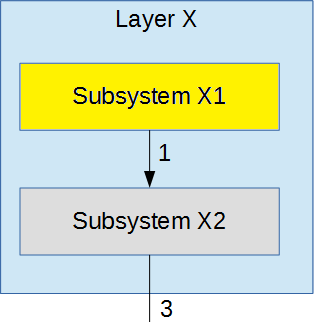
\includegraphics[width=0.60\textwidth]{images/subsystem}
 \caption{Example Daughter Board - BRD diagram}
\end{figure}

\subsubsection{Assumptions}
The BRD should communicate without any issues (like a BUS connection).

\subsubsection{Responsibilities}
The Base BRD Connector is used to interface between the daughter board and the MIPI Camera BRD Connector on the Cypress CX3 Board and vice versa.

\subsubsection{Subsystem Interfaces}
This connector contains 52 pins, but not all of the pins will be used. This connector is directly connected to the camera module connector in order to transfer the data back and forth at a faster rate.  Throughout this connector, multiple pins receive different types of voltages in order to perform different tasks. For complexity issues, the Base BRD Connector will be connected to the bottom layer of the Daughter Board.

\begin {table}[H]
\caption {Subsystem interfaces}
\begin{center}
    \begin{tabular}{ | p{1cm} | p{6cm} | p{3cm} | p{3cm} |}
    \hline
    ID & Description & Inputs & Outputs \\ \hline
     \#01 & MIPI Controls & \pbox{3cm}{Input 1 - SCL \\ Input 2 - SDA} & \pbox{3cm}{Output 1 - MIPI Data \\ Output 2 - MIPI Clock \\ Output 3 - MIPI Power \\ Output 4 - SDA}  \\ \hline
    \end{tabular}
\end{center}
\end{table}

\subsection{MIPI Camera}
The camera module used for the Eye Tracker system is a 5MP pcDuino camera that will be used to capture data for processing. The pcDuino camera uses the OV5640 image sensor.

\begin{figure}[h!]
	\centering
 	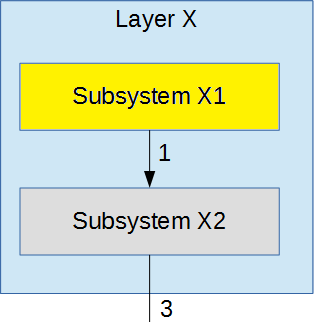
\includegraphics[width=0.60\textwidth]{images/subsystem}
 \caption{Example Daughter Board - Camera Module diagram}
\end{figure}

\subsubsection{Assumptions}
The camera module will capture image and video at least 30FPS at 5MP.

\subsubsection{Responsibilities}
This image sensor is capable of capturing 2592x1944 active array of image and video at a minimum of 30 FPS. Since this new camera uses the OV5640, it is compatible with the Cypress CX3.

\subsubsection{Subsystem Interfaces}

The camera uses the OV5640 image sensor, which is a high quality CMOS image sensor.

\begin {table}[H]
\caption {Subsystem interfaces}
\begin{center}
    \begin{tabular}{ | p{1cm} | p{6cm} | p{3cm} | p{3cm} |}
    \hline
    ID & Description & Inputs & Outputs \\ \hline
    \#01 & CMOS Data from Camera & \pbox{3cm}{Input 1 - SCL \\ Input 2 - SDA} & \pbox{3cm}{Output 1 - Data \\ Output 2 - Clock \\ Output 3 - SDA}  \\ \hline
    \end{tabular}
\end{center}
\end{table}

\subsection{CMOS-MIPI Converter}
The camera connector is new, and will be replacing the camera connector that was on the CX3 development board. The new connector allows for the use of the pcDuino camera module. This where the camera performs a CMOS to MIPI conversion in order to transfer the data collected from the camera module.

\begin{figure}[h!]
	\centering
 	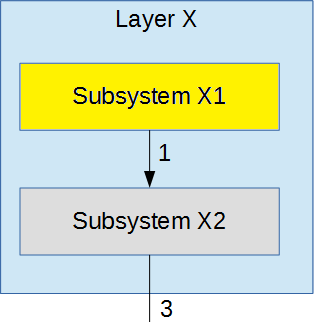
\includegraphics[width=0.60\textwidth]{images/subsystem}
 \caption{Example Daughter Board - Camera Connector diagram}
\end{figure}

\subsubsection{Assumptions}
The camera connector is compatible with the new module and the BRD.

\subsubsection{Responsibilities}
The camera connector is used to connect the camera module to the daughter board and transfer the data that the camera captures to the Base BRD Connector.

\subsubsection{Subsystem Interfaces}
In order for the camera module to function properly with the Cypress CX3, it received different voltage inputs in different pins. The datasheet of the OV5640 (Image Sensor) in order to determine which pins will be used on the camera connector and where to connect each pin at the Base BRD Connector. Since this camera will only be used for eye tracking purposes only, the user will not be able to reset the camera since we disabled the reset pin on the camera connector.

\begin {table}[H]
\caption {Subsystem interfaces}
\begin{center}
    \begin{tabular}{ | p{1cm} | p{6cm} | p{3cm} | p{3cm} |}
    \hline
    ID & Description & Inputs & Outputs \\ \hline
    \#01 & Camera Connector & \pbox{3cm}{Input 1 - MIPI Data \\ Input 2 - MIPI Clock \\ Input 3 - SDA} & \pbox{3cm}{Output 1 - Converted Data \\ Output 2 - Camera Clock Signal \\ Output 3 - SDA}  \\ \hline
    \end{tabular}
\end{center}
\end{table}
